%%%%%%%%%%%%%%%%%%%%%%%%%%%%%%%%%%%%%%%%%%%%%%%%%%%%
%% P S E U D O - R A N D O M    G E N E R A T O R %%
%%%%%%%%%%%%%%%%%%%%%%%%%%%%%%%%%%%%%%%%%%%%%%%%%%%%

\subsection{Pseudo-Random Generator}
\label{subsec:prg}

The Pseudo-Random Generator is responsible for generating a candidate (victim way) used by the \EvictingBlock during cache line replacement. The generator is based on a \textit{Linear Feedback Shift Register} (LFSR), which provides a compact hardware implementation for generating pseudo-random sequences.

\begin{figure}[h]
	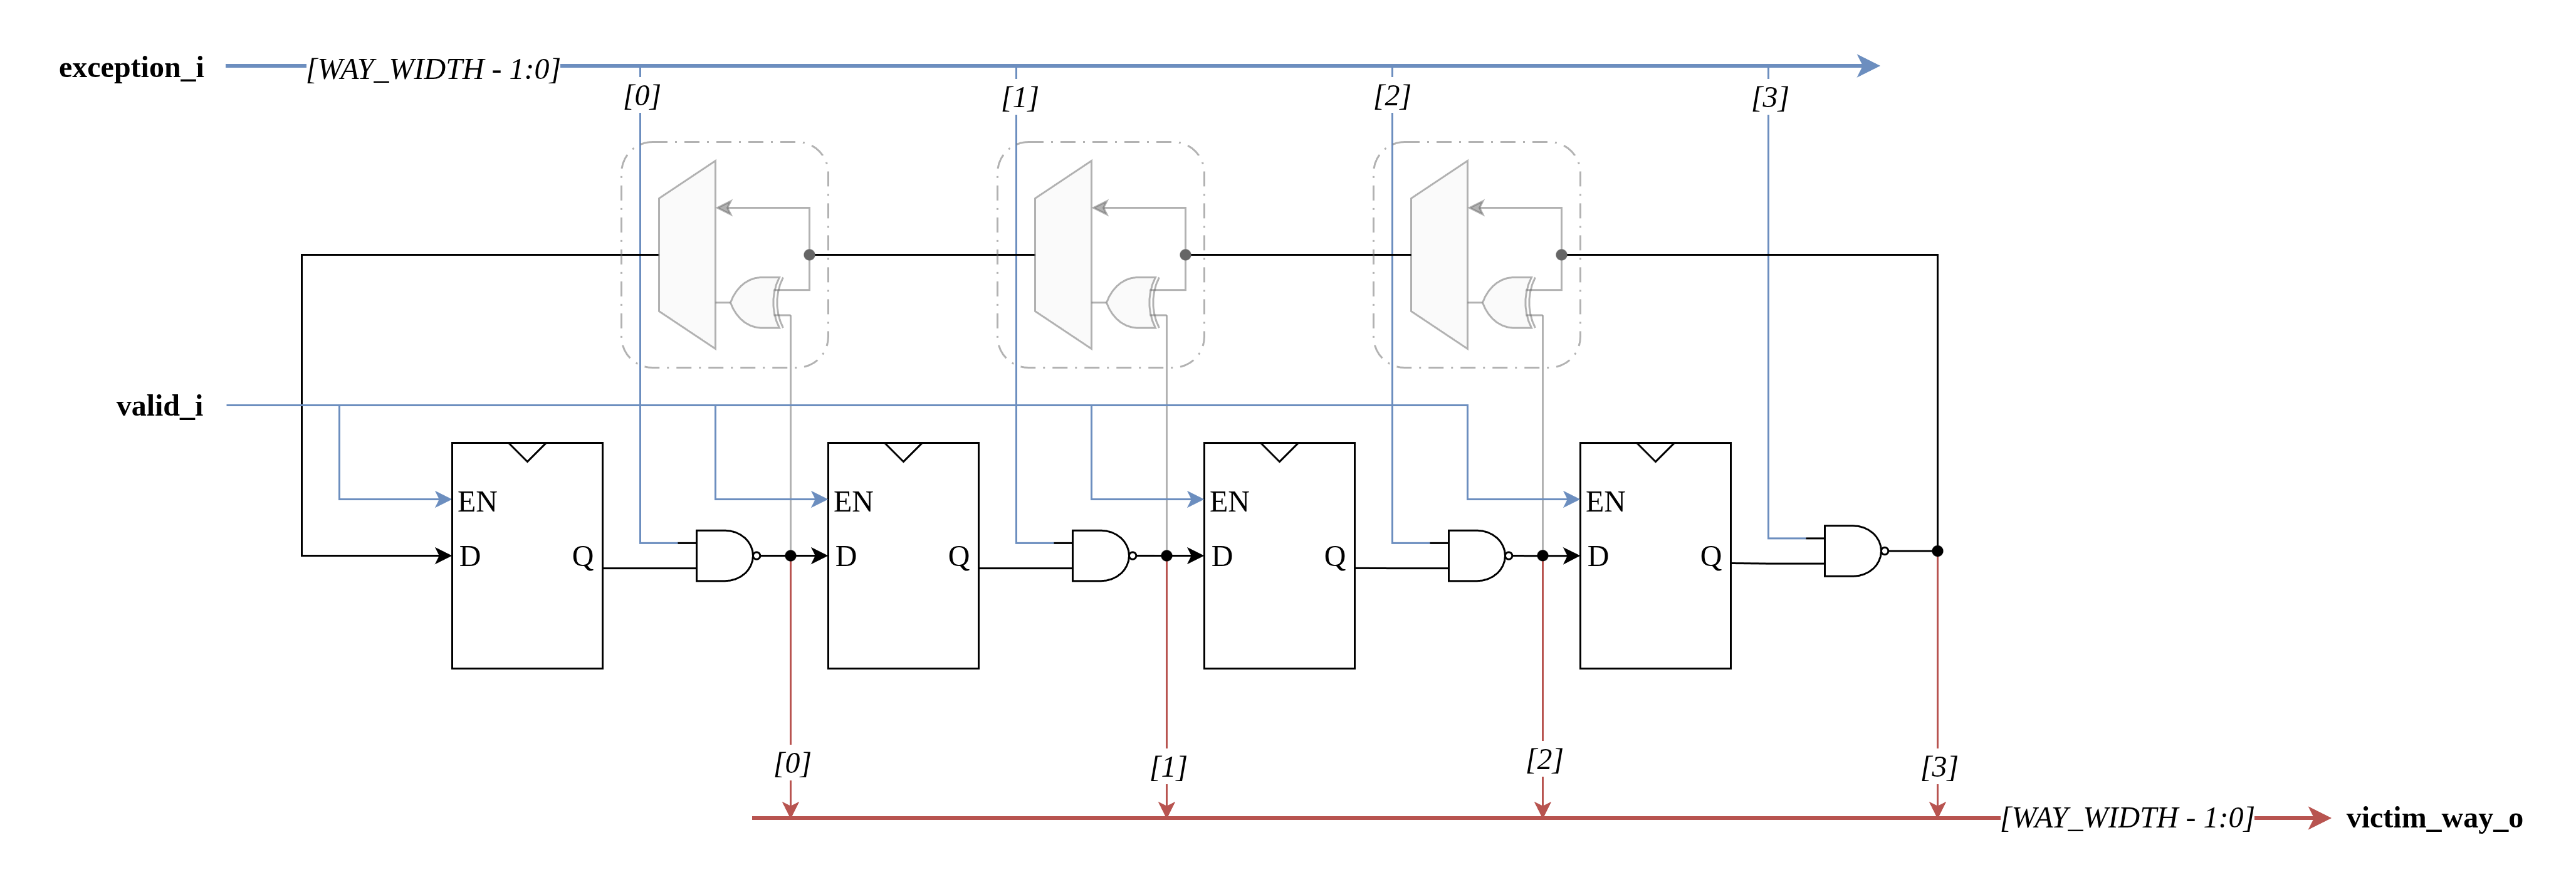
\includegraphics[width=16cm]{PRG.png}
	\caption{Pseudo-Random Generator scheme}
\end{figure}

\begin{table}[htbp]
	\centering
	\small
	\begin{tabularx}{\textwidth}{l c c X}
		\toprule
		\textbf{Parameter} & \textbf{Valid Range} & \textbf{Default} & \textbf{Description} \\
		\midrule
		
		\verb|LFSR_WIDTH| &
		Positive integer &
		\verb|WAY_WIDTH| &
		Number of flip-flops in the LFSR. \\
		
		\verb|LFSR_POLY| &
		Configurable &
		--- &
		Selects the feedback polynomial used by the LFSR. \\
		
		\bottomrule
	\end{tabularx}
	\caption{LFSR configuration parameters}
	\label{tab:lfsr_parameters}
\end{table}
	

\begin{table}[htbp]
	\centering
	\label{tab:prg_ports}
	\small
	\begin{tabularx}{\textwidth}{l c c X}
		\toprule
		\textbf{Ports} & \textbf{Direction} & \textbf{Width} & \textbf{Description} \\
		\midrule
		\verb| exception_i | & Input & \verb| WAY_WIDTH | & Way index that must be excluded from the generated victim way. \\
		\verb| valid_i | & Input & \verb| 1 | & Indicates whether the selected exception way is valid. \\
		\verb| victim_way_o | & Output & \verb| WAY_WIDTH | & Pseudo-randomly generated way index selected as the victim way. \\
		\bottomrule
	\end{tabularx}
	\caption{Pseudo-Random Generator ports}
\end{table}

For a cache with \verb|WAY_NUM| ways, the minimum LFSR width is

\begin{equation}
	N = \log_2( \verb| WAY_NUM |)
\end{equation}

flip-flops. The feedback function of the LFSR is configurable, allowing different feedback polynomials to be selected. The polynomial configuration is implemented using multiplexers placed between adjacent stages of the shift register. For the $i$-th polynomial coefficient, the corresponding multiplexer determines whether the feedback path contains an XOR operation or a direct connection.

The NAND-based transformation provides a simple mechanism for modifying the generated value when it coincides with the prohibited way. If a generated bit matches the corresponding bit of the prohibited way, the NAND logic inverts the affected bit. Therefore, if the complete generated victim way coincides with the prohibited way, the corresponding matching bits are inverted, resulting in a different way index.

The NAND-based feedback also prevents the LFSR from becoming permanently locked in the all-zero state. In a conventional LFSR, the state consisting entirely of zeros is a lock-up state: since all feedback values remain zero, the register cannot transition to another state. In the proposed design, the feedback logic additionally depends on the prohibited way index. Even when the generated way and the prohibited way do not completely match, any matching individual bits can still be inverted by the NAND logic. Consequently, when the LFSR reaches the all-zero state, the interaction with the prohibited way can introduce non-zero bits into the next LFSR state. Therefore, the generator can leave the conventional all-zero lock-up state without requiring separate zero-state recovery logic.

\begin{warningbox}{Victim Way Distribution}
	The NMRU replacement policy relies on the pseudo-random generator providing a sufficiently uniform distribution of victim ways. Ideally, each possible way index should have approximately the same probability of being generated.
	
	This property is not guaranteed by the proposed generator architecture. In the proposed implementation, additional NAND logic is introduced between the LFSR stages to account for the prohibited way. This modification changes the state transition function of the original LFSR and can therefore introduce a bias into the distribution of generated victim ways.
	
	Therefore, before configuring the cache parameters (\verb|SET_NUM|, \verb|WAY_NUM|), the distribution of the generated victim way values must be verified for the selected LFSR configuration. The verification should include a sufficiently long generated sequence and should confirm that all valid way indices occur with approximately equal frequency.
	
	If a significant bias is observed, the distribution can be adjusted by selecting a different feedback polynomial. Another possible solution is to increase the length of the LFSR.
\end{warningbox}